% Options for packages loaded elsewhere
\PassOptionsToPackage{unicode}{hyperref}
\PassOptionsToPackage{hyphens}{url}
\documentclass[
  ignorenonframetext,
]{beamer}
\newif\ifbibliography
\usepackage{pgfpages}
\setbeamertemplate{caption}[numbered]
\setbeamertemplate{caption label separator}{: }
\setbeamercolor{caption name}{fg=normal text.fg}
\beamertemplatenavigationsymbolsempty
% remove section numbering
\setbeamertemplate{part page}{
  \centering
  \begin{beamercolorbox}[sep=16pt,center]{part title}
    \usebeamerfont{part title}\insertpart\par
  \end{beamercolorbox}
}
\setbeamertemplate{section page}{
  \centering
  \begin{beamercolorbox}[sep=12pt,center]{section title}
    \usebeamerfont{section title}\insertsection\par
  \end{beamercolorbox}
}
\setbeamertemplate{subsection page}{
  \centering
  \begin{beamercolorbox}[sep=8pt,center]{subsection title}
    \usebeamerfont{subsection title}\insertsubsection\par
  \end{beamercolorbox}
}
% Prevent slide breaks in the middle of a paragraph
\widowpenalties 1 10000
\raggedbottom
\AtBeginPart{
  \frame{\partpage}
}
\AtBeginSection{
  \ifbibliography
  \else
    \frame{\sectionpage}
  \fi
}
\AtBeginSubsection{
  \frame{\subsectionpage}
}
\usepackage{iftex}
\ifPDFTeX
  \usepackage[T1]{fontenc}
  \usepackage[utf8]{inputenc}
  \usepackage{textcomp} % provide euro and other symbols
\else % if luatex or xetex
  \usepackage{unicode-math} % this also loads fontspec
  \defaultfontfeatures{Scale=MatchLowercase}
  \defaultfontfeatures[\rmfamily]{Ligatures=TeX,Scale=1}
\fi
\usepackage{lmodern}
\ifPDFTeX\else
  % xetex/luatex font selection
\fi
% Use upquote if available, for straight quotes in verbatim environments
\IfFileExists{upquote.sty}{\usepackage{upquote}}{}
\IfFileExists{microtype.sty}{% use microtype if available
  \usepackage[]{microtype}
  \UseMicrotypeSet[protrusion]{basicmath} % disable protrusion for tt fonts
}{}
\makeatletter
\@ifundefined{KOMAClassName}{% if non-KOMA class
  \IfFileExists{parskip.sty}{%
    \usepackage{parskip}
  }{% else
    \setlength{\parindent}{0pt}
    \setlength{\parskip}{6pt plus 2pt minus 1pt}}
}{% if KOMA class
  \KOMAoptions{parskip=half}}
\makeatother
\usepackage{longtable,booktabs,array}
\usepackage{caption}
\captionsetup[table]{skip=6pt}
\newcounter{none} % for unnumbered tables
\usepackage{calc} % for calculating minipage widths
\usepackage{caption}
% Make caption package work with longtable
\makeatletter
\def\fnum@table{\tablename~\thetable}
\makeatother
\usepackage{graphicx}
\makeatletter
\newsavebox\pandoc@box
\newcommand*\pandocbounded[1]{% scales image to fit in text height/width
  \sbox\pandoc@box{#1}%
  \Gscale@div\@tempa{\textheight}{\dimexpr\ht\pandoc@box+\dp\pandoc@box\relax}%
  \Gscale@div\@tempb{\linewidth}{\wd\pandoc@box}%
  \ifdim\@tempb\p@<\@tempa\p@\let\@tempa\@tempb\fi% select the smaller of both
  \ifdim\@tempa\p@<\p@\scalebox{\@tempa}{\usebox\pandoc@box}%
  \else\usebox{\pandoc@box}%
  \fi%
}
% Set default figure placement to htbp
\def\fps@figure{htbp}
\makeatother
\setlength{\emergencystretch}{3em} % prevent overfull lines
\providecommand{\tightlist}{%
  \setlength{\itemsep}{0pt}\setlength{\parskip}{0pt}}
% Auto-generated by infrastructure/rendering/_pdf_latex_helpers.py::extract_math_font_preamble.
% Minimal header passed to Pandoc via -H so Beamer slides pick up the same math font
% as the combined-PDF path. Adjust the manuscript's preamble.md to change the font globally.
\usepackage{unicode-math}
\setmathfont{latinmodern-math.otf}

% Slide layout defaults for warning-clean scientific decks.
\usepackage{etoolbox}
\IfFileExists{xurl.sty}{\usepackage{xurl}}{}
\IfFileExists{seqsplit.sty}{\usepackage{seqsplit}}{\newcommand{\seqsplit}[1]{#1}}
\protected\def\breakseq#1{\seqsplit{#1}}
\protected\def\breaktt#1{\begingroup\ttfamily\seqsplit{#1}\endgroup}
\setlength{\emergencystretch}{6em}
\tolerance=5000
\hbadness=10000
\hfuzz=1pt
\setlength{\tabcolsep}{2pt}
\AtBeginEnvironment{longtable}{\tiny\renewcommand{\arraystretch}{0.86}\setlength{\tabcolsep}{1pt}}
\AtBeginEnvironment{tabular}{\tiny\renewcommand{\arraystretch}{0.86}\setlength{\tabcolsep}{1pt}}
\AtBeginEnvironment{equation}{\tiny}
\AtBeginEnvironment{equation*}{\tiny}
\AtBeginEnvironment{align}{\tiny}
\AtBeginEnvironment{align*}{\tiny}
\AtBeginEnvironment{itemize}{\footnotesize}
\AtBeginEnvironment{enumerate}{\footnotesize}
\AtBeginEnvironment{description}{\footnotesize}
\setbeamerfont{caption}{size=\tiny}
\setbeamerfont{caption name}{size=\tiny}
\setbeamerfont{normal text}{size=\small}
\setbeamerfont{frametitle}{size=\small}
\setbeamerfont{section title}{size=\footnotesize}
\setbeamerfont{subsection title}{size=\footnotesize}
\setbeamertemplate{section page}{%
  \centering
  \begin{beamercolorbox}[sep=12pt,center,wd=\paperwidth]{section title}
    \parbox{0.86\paperwidth}{\centering\usebeamerfont{section title}\insertsection\par}
  \end{beamercolorbox}
}
\setbeamertemplate{subsection page}{%
  \centering
  \begin{beamercolorbox}[sep=8pt,center,wd=\paperwidth]{subsection title}
    \parbox{0.86\paperwidth}{\centering\usebeamerfont{subsection title}\insertsubsection\par}
  \end{beamercolorbox}
}
\setlength{\abovecaptionskip}{2pt}
\setlength{\belowcaptionskip}{0pt}

% Natbib and cross-reference fallbacks — slides don't load natbib
% or cleveref, but combined-PDF manuscript prose may emit these
% commands. The fallback renders citations as a bracketed key list
% and cross-references as detokenized labels so slides don't fail on
% undefined control sequences or raw underscores. \providecommand is
% a no-op if packages load later.
\providecommand{\citep}[1]{[#1]}
\providecommand{\citet}[1]{#1}
\providecommand{\citealp}[1]{#1}
\providecommand{\citeauthor}[1]{#1}
\providecommand{\citeyear}[1]{#1}
\providecommand{\cref}[1]{\texttt{\detokenize{#1}}}
\providecommand{\Cref}[1]{\texttt{\detokenize{#1}}}

\newtheorem{proposition}{Proposition}
\newtheorem{hypothesis}{Hypothesis}
\usepackage{bookmark}
\IfFileExists{xurl.sty}{\usepackage{xurl}}{} % add URL line breaks if available
\urlstyle{same}
% fallback for those not using the hyperref driver hyperxmp:
\makeatletter
\@ifundefined{xmpquote}{\newcommand{\xmpquote}[1]{#1}}{}
\makeatother
\hypersetup{
  hidelinks,
  pdfcreator={LaTeX via pandoc}}

\author{\texorpdfstring{}{}}
\date{}

\begin{document}

\section{Discussion and Conclusion: What the Artifact Establishes---and
What It Does
Not}\label{discussion-and-conclusion-what-the-artifact-establishesand-what-it-does-not}

\begin{frame}[allowframebreaks]{Principal findings: a claim-calibrated
curriculum artifact}
\protect\phantomsection\label{principal-findings-a-claim-calibrated-curriculum-artifact}
Active Skillference establishes a bounded engineering result: a
contested formal subject can be represented as an inspectable
prerequisite graph whose structural, quantitative, scholarly, and
delivery contracts are checked separately. The curriculum graph is a
validated DAG; learner-facing computed values are resolved from tested
kernels; citations are assigned source roles; and generated figures,
manuscript references, and SkillTree payloads are audited as connected
artifacts. These are properties of this checkout and its build process,
not evidence that the selected order is optimal for every learner or
that the underlying scientific framework is empirically confirmed.
\end{frame}

\begin{frame}[allowframebreaks]{Interpretation: infrastructure rather
than intelligence or personalization}
\protect\phantomsection\label{interpretation-infrastructure-rather-than-intelligence-or-personalization}
The mathematical examples and the curriculum infrastructure operate at
different levels. The kernels implement small, model-dependent
demonstrations of inference and policy evaluation. The curriculum layer
orders and assesses concepts. The provenance layer records how values
and sources enter the learner-facing artifact. None of these layers is
an intelligent tutor, a general-purpose reasoning system, or an adaptive
learner model. In particular, the term \emph{agent} in the mathematical
examples refers to a formal model with specified states, observations,
preferences, and policies; it should not be read as a claim about
consciousness, general intelligence, autonomy, or human-like learning.

\end{frame}

\begin{frame}[allowframebreaks]{Interpretation: infrastructure rather
than intelligence or personalization}
The related-work literature supports this separation. Active Inference
formulations can connect belief updating, action selection, learning,
and epistemic behavior, but their predictions depend on the generative
model, preferences, approximation, and policy set (Rao and Ballard 1999;
Friston 2013, 2019; Ramstead et al. 2018). The supplement therefore
keeps the VFE/EFE derivations, sign conventions, and preference
assumptions visible instead of treating one computed policy comparison
as a universal account of intelligent behavior. Learner-state models
such as knowledge tracing and Q-matrix cognitive diagnosis belong to a
separate adaptive-learning evidence layer and are cited here as
comparison boundaries, not as components of this artifact (Piech et al.
2015; Tao et al. 2024).
\end{frame}

\begin{frame}[allowframebreaks]{Implications: future adaptive learning
systems and open-science interoperability}
\protect\phantomsection\label{implications-future-adaptive-learning-systems-and-open-science-interoperability}
The delivery contract is useful precisely because it does not hide
ownership boundaries. The exporter creates a SkillTree-compatible
Project -\textgreater{} Subject -\textgreater{} Skill profile with
learning-path dependencies and quiz associations. The local dashboard
exposes generated artifacts and opens official subject and quiz routes,
while SkillTree remains the owner of progress, ranking, scoring,
completion, and authentication. This makes the repository a candidate
foundation for a later adaptive study, not an adaptive system in the
present release.

\end{frame}

\begin{frame}[allowframebreaks]{Implications: future adaptive learning
systems and open-science interoperability}
A genuinely adaptive extension would require learner response data, a
validated model of learner state, a transparent rule for selecting the
next skill, item-level measurement, privacy and consent controls, and
prospective evaluation against a preregistered comparator (Doignon and
Falmagne 1985; Fu and Fang 2025; Design-Based Research Collective 2003;
Liu and Khalil 2023; Piech et al. 2015; Tao et al. 2024). Knowledge
tracing and Q-matrix cognitive diagnosis are comparison literatures for
those stronger commitments, not components of the present export.
Provenance and graph validation would remain necessary infrastructure,
but they would not by themselves establish personalization quality or
learning effectiveness.

\end{frame}

\begin{frame}[allowframebreaks]{Implications: future adaptive learning
systems and open-science interoperability}
The community contribution should be read at the same bounded level. The
Active Inference Institute's public website repository presents a public
resource hub for learning, research, participation, and contribution,
with public repositories and a documented boundary between internal
inputs and verified public projections (Active Inference Institute
2026). Active Skillference contributes a complementary artifact to that
open-science environment: it packages a prerequisite graph,
kernel-backed examples, source-role audit, and SkillTree handoff into a
rerunnable educational release. The relationship is interoperable and
community-facing, not institutional: this repository does not claim to
be an Institute product, an official curriculum, or an endorsement of
any contributor or public pathway.
\end{frame}

\begin{frame}[fragile,allowframebreaks]{Limitations and planned
empirical evaluation}
\protect\phantomsection\label{limitations-and-planned-empirical-evaluation}
The release state is machine-readable. As of 2026-07-31,
\texttt{tasks.yaml} records 78 roadmap tasks: 74 completed milestones
and 4 open items across metadata, skilltree, validation.
\texttt{TODO.md} is rendered from the same source.
fig.~\ref{fig:roadmap_risk} shows the current distribution of open
versus completed work by surface and release class, keeping
release-readiness language tied to the validator state that drives the
roadmap.

\end{frame}

\begin{frame}[fragile,allowframebreaks]{Limitations and planned
empirical evaluation}
\begin{figure}
\centering
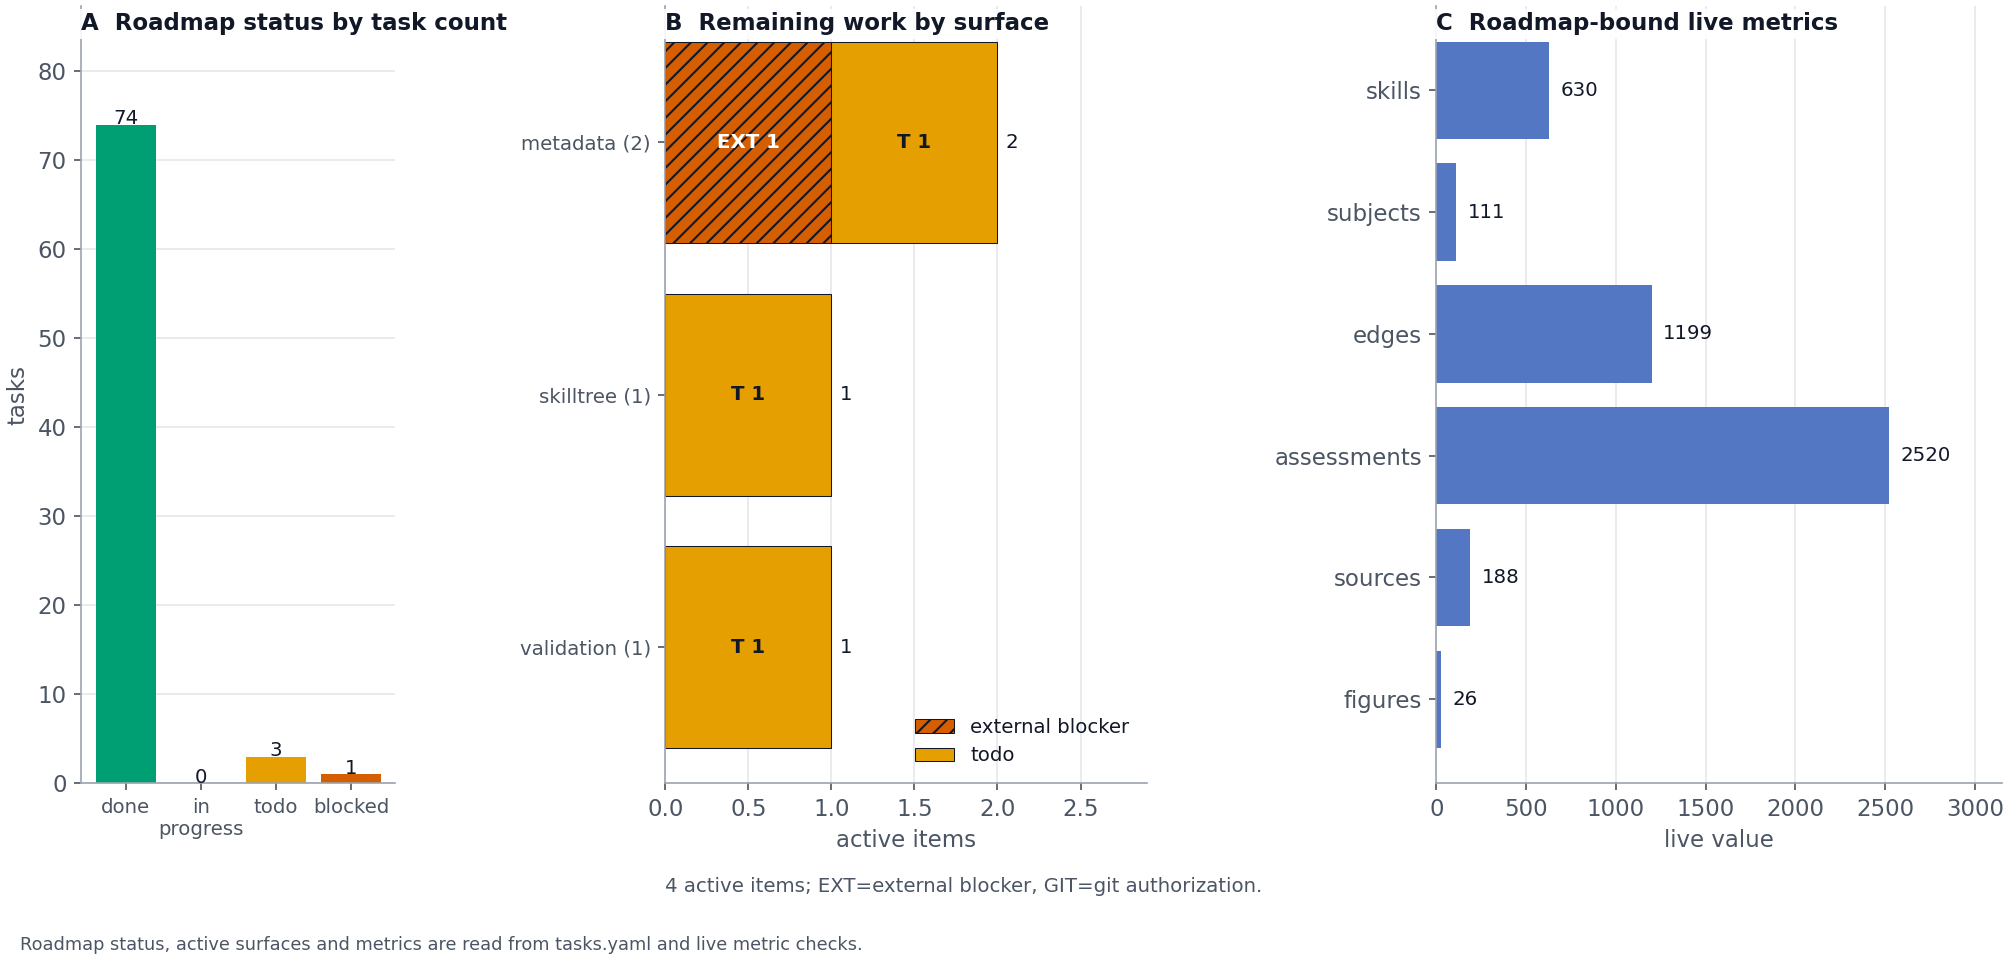
\includegraphics[width=0.88\linewidth,height=0.40\textheight,keepaspectratio,alt={Roadmap status by artifact surface generated from tasks.yaml and the live metrics stored in the roadmap source data. The first panel counts roadmap items by status, the middle panel groups remaining open or blocked work by surface and release class with direct EXT/GIT segment labels, hatching, and surface totals, and the final panel reports current curriculum, assessment, scholarship, and figure metrics. The figure separates external blockers from git-authorization hygiene using machine-readable roadmap data, so release-readiness text must agree with the same source.}]{../figures/roadmap_risk.png}
\caption{Roadmap status by artifact surface generated from
\protect\texttt{tasks.yaml} and the live metrics stored in the roadmap
source data. The first panel counts roadmap items by status, the middle
panel groups remaining open or blocked work by surface and release class
with direct EXT/GIT segment labels, hatching, and surface totals, and
the final panel reports current curriculum, assessment, scholarship, and
figure metrics. The figure separates external blockers from
git-authorization hygiene using machine-readable roadmap data, so
release-readiness text must agree with the same
source.}\label{fig:roadmap_risk}
\end{figure}

\end{frame}

\begin{frame}[fragile,allowframebreaks]{Limitations and planned
empirical evaluation}
The limitations are therefore substantive rather than cosmetic. The
kernels cover fixed, small discrete teaching cases and bounded
predictive-coding or planning demonstrations; their conclusions depend
on the stated model, preferences, inputs, and approximation regime. The
runtime depends on SkillTree for live progress and quiz state, and this
release contains no learner-response data, learner-state inference,
retention measure, transfer measure, efficacy estimate, or
differential-benefit analysis. The planned pilot described in
sec.~13 and
the fuller boundary analysis in
sec.~19 define
the evidence needed before those claims can be made.
\end{frame}

\begin{frame}[allowframebreaks]{Conclusion: a bounded, reproducible
contribution}
\protect\phantomsection\label{conclusion-a-bounded-reproducible-contribution}
The strongest conclusion is narrower and more useful: Active
Skillference makes the construction, provenance, and delivery of a
formal Active Inference curriculum more inspectable, reproducible, and
auditable. It establishes an infrastructure artifact and an
open-science-compatible handoff surface; it does not establish
intelligent tutoring, personalization, learner improvement, or empirical
confirmation of the Free Energy Principle.
\end{frame}

\end{document}
